Estas ondas dan la impresión de vibrar en el mismo lugar de forma fija. Son el resultado de la superposición de dos ondas viajeras que se mueven en direcciones opuestas. Los \textbf{nodos} son puntos que permanecen inmóviles, mientras que los \textbf{antinodos} oscilan.

\begin{grafica}[H]
\centering
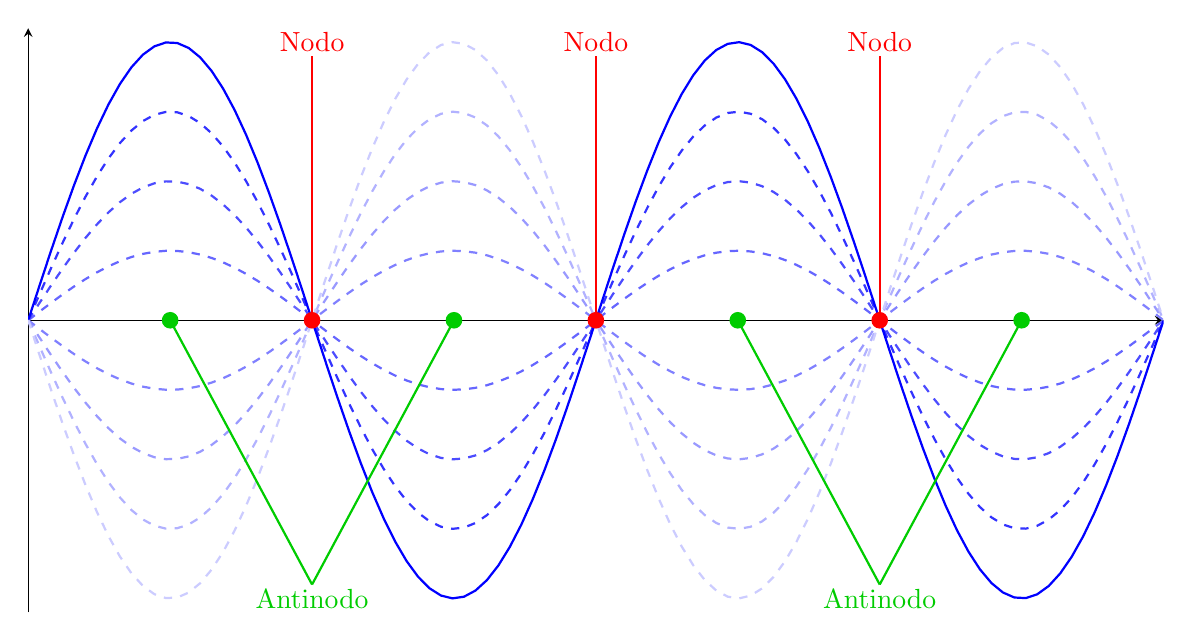
\begin{tikzpicture}
  \begin{axis}[
    xmin=0,xmax=4*pi,
    ymin=-4.2,ymax=4.2,
    axis lines=middle,
    xtick={0},ytick={0},
    width=16cm,height=9cm
    ]

    % sin
    \addplot[color=blue!60!white,samples=100,domain=0:4*pi,thick,dashed]{sin(deg(x))};
    \addplot[color=blue!70!white,samples=100,domain=0:4*pi,thick,dashed]{2*sin(deg(x))};
    \addplot[color=blue!80!white,samples=100,domain=0:4*pi,thick,dashed]{3*sin(deg(x))};
    \addplot[color=blue,samples=100,domain=0:4*pi,thick]{4*sin(deg(x))};

    % cos
    \addplot[color=blue!50!white,samples=100,domain=0:4*pi,thick,dashed]{-sin(deg(x))};
    \addplot[color=blue!40!white,samples=100,domain=0:4*pi,thick,dashed]{-2*sin(deg(x))};
    \addplot[color=blue!30!white,samples=100,domain=0:4*pi,thick,dashed]{-3*sin(deg(x))};
    \addplot[color=blue!20!white,samples=100,domain=0:4*pi,thick,dashed]{-4*sin(deg(x))};

    % nodo 1
    \fill[red] (axis cs:pi,0) circle[radius=3pt];
    \draw[red,thick] (axis cs:pi,0) -- (axis cs:pi,3.8);
    \node[red,thick] at (axis cs:pi,4) {Nodo};

    % nodo 2
    \fill[red] (axis cs:2*pi,0) circle[radius=3pt];
    \draw[red,thick] (axis cs:2*pi,0) -- (axis cs:2*pi,3.8);
    \node[red,thick] at (axis cs:2*pi,4) {Nodo};

    % nodo 3
    \fill[red] (axis cs:3*pi,0) circle[radius=3pt];
    \draw[red,thick] (axis cs:3*pi,0) -- (axis cs:3*pi,3.8);
    \node[red,thick] at (axis cs:3*pi,4) {Nodo};

    % antinodo 1
    \fill[green!80!black] (axis cs:pi/2,0) circle[radius=3pt];
    \draw[green!80!black,thick] (axis cs:pi/2,0) -- (axis cs:pi,-3.8);
    % antinodo 2
    \fill[green!80!black] (axis cs:3*pi/2,0) circle[radius=3pt];
    \draw[green!80!black,thick] (axis cs:3*pi/2,0) -- (axis cs:pi,-3.8);
    % antinodo 1-2
    \node[green!80!black,thick] at (axis cs:pi,-4) {Antinodo};

    % antinodo 3
    \fill[green!80!black] (axis cs:5*pi/2,0) circle[radius=3pt];
    \draw[green!80!black,thick] (axis cs:5*pi/2,0) -- (axis cs:3*pi,-3.8);
    % antinodo 4
    \fill[green!80!black] (axis cs:7*pi/2,0) circle[radius=3pt];
    \draw[green!80!black,thick] (axis cs:7*pi/2,0) -- (axis cs:3*pi,-3.8);
    % antinodo 3-4
    \node[green!80!black,thick] at (axis cs:3*pi,-4) {Antinodo};
  \end{axis}
\end{tikzpicture}
\caption{Onda estacionaria}
\end{grafica}

Ejemplos:

\begin{itemize}
  \item Cuerdas, en instrumentos musicales como la guitarra.
  \item Tubos sonoros, en instrumentos como la flauta o el órgano.
\end{itemize}
